% !TEX root = ../../../main.tex
% 来源：高中物理甲种本·第二册（热学·电学）
% 章节：固体和液体的性质 / 空间点阵
% 原始文件：4.tex，行 51-111
% 类型：tikz
% ---
	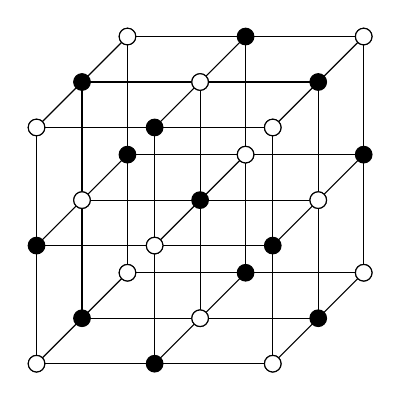
\begin{tikzpicture}[>=stealth, scale=1.5 ]
%\draw [->](0,0,0)--(0,0,10)node [right]{$z$};
%\draw [->](0,0,0)--(0,10,0)node [right]{$y$};
%\draw [->](0,0,0)--(10,0,0)node [right]{$x$};

%\draw (0,0,0) circle (2pt);
%\draw (0,0,2) circle (2pt);

\draw (0,0,0)--(0,0,2);
\draw (0,0,0)--(0,2,0);
\draw (0,0,0)--(2,0,0);
\draw (0,1,0)--(0,1,2);
\draw (0,1,0)--(2,1,0);
\draw (0,2,0)--(0,2,2);
\draw (0,2,0)--(2,2,0);
\draw (1,1,0)--(1,1,2);
\draw (1,2,0)--(1,2,2);
\draw (2,1,0)--(2,1,2);
\draw (2,2,0)--(2,2,2);
\draw (1,0,0)--(1,0,2);
\draw (1,0,0)--(1,2,0);
\draw (2,0,0)--(2,0,2);
\draw (2,0,0)--(2,2,0);
\draw(0,2,1)--(2,2,1);
\draw(0,2,2)--(2,2,2);
\draw(0,1,1)--(2,1,1);
\draw(0,1,2)--(2,1,2);
\draw (0,2,2)--(0,0,2);
\draw (2,0,2)--(0,0,2);
\draw (2,0,1)--(0,0,1);
\draw (2,0,2)--(2,2,2);
\draw (2,0,1)--(2,2,1);
\draw (1,0,1)--(1,2,1);
\draw (1,0,2)--(1,2,2);
\draw (0,0,1)--(0,2,1);


\foreach \x in {0,1,2}
\foreach \y in {0,1,2}
\foreach \z in {0,1,2}
{
\draw [fill=black](\x,\y,\z) circle (2pt);
}


\draw [fill=white] ( 0,0,0 )  circle (2pt);
\draw [fill=white] ( 0,0,2 )  circle (2pt);
\draw [fill=white] ( 0,1,1 )  circle (2pt);
\draw [fill=white] ( 1,0,1 )  circle (2pt);
\draw [fill=white] ( 2,0,0 )  circle (2pt);
\draw [fill=white] ( 2,0,2 )  circle (2pt);
\draw [fill=white] ( 2,1,1 )  circle (2pt);
\draw [fill=white] ( 1,2,1 )  circle (2pt);
\draw [fill=white] ( 0,2,0 )  circle (2pt);
\draw [fill=white] ( 0,2,2 )  circle (2pt);
\draw [fill=white] ( 1,1,0 )  circle (2pt);
\draw [fill=white] ( 1,1,2 )  circle (2pt);
\draw [fill=white] ( 2,2,0 )  circle (2pt);
\draw [fill=white] ( 2,2,2 )  circle (2pt);

\end{tikzpicture}
